% !TEX encoding = UTF-8
% !TEX TS-program = xelatex

\documentclass[a4paper,10pt]{article}
%A Few Useful Packages
\usepackage{marvosym}
\usepackage{fontspec} 					%for loading fonts
\usepackage{xunicode,xltxtra,url,parskip} 	%other packages for formatting
\RequirePackage{color,graphicx}
\usepackage[usenames,dvipsnames]{xcolor}
\usepackage[big]{layaureo} 				%better formatting of the A4 page
% an alternative to Layaureo can be ** \usepackage{fullpage} **
\usepackage{supertabular} 				%for Grades
\usepackage{titlesec}					%custom \section
\usepackage{float}

%Setup hyperref package, and colours for links
\usepackage{hyperref}
\definecolor{linkcolour}{rgb}{0,0.2,0.6}
\hypersetup{colorlinks,breaklinks,urlcolor=linkcolour, linkcolor=linkcolour}

%FONTS
\defaultfontfeatures{Mapping=tex-text}
%\setmainfont[SmallCapsFont = Fontin SmallCaps]{Fontin}
%%% modified for Karol Kozioł for ShareLaTeX use
\setmainfont[
Path = font/ ,
SmallCapsFont = Fontin-SmallCaps.otf,
BoldFont = Fontin-Bold.otf,
ItalicFont = Fontin-Italic.otf
]
{Fontin.otf}

\titleformat{\section}{\Large\scshape\raggedright}{}{0em}{}[\titlerule]
\titlespacing{\section}{0pt}{3pt}{3pt}
%Tweak a bit the top margin
%\addtolength{\voffset}{-1.3cm}

%Italian hyphenation for the word: ''corporations''
\hyphenation{im-pre-se}

%-------------WATERMARK TEST [**not part of a CV**]---------------
\usepackage[absolute]{textpos}

\setlength{\TPHorizModule}{30mm}
\setlength{\TPVertModule}{\TPHorizModule}
\textblockorigin{2mm}{0.65\paperheight}
\setlength{\parindent}{0pt}

%--------------------BEGIN DOCUMENT----------------------
\begin{document}

\pagestyle{empty} % non-numbered pages

\newcommand{\name}{Luca}
\newcommand{\surname}{Allegro}

\newcommand{\head}{
	%--------------------TITLE-------------
	\par{\centering
		\huge{ \name{} \textsc{\surname{}}}
		\begin{figure}[h!]
			\centering
			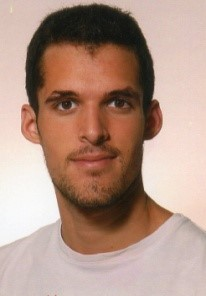
\includegraphics{img/foto_tessera}
		\end{figure}
		\bigskip\par
	}
}

\newcommand{\personalData}[2]{\textsc{#1:} & #2 \\}

\newcommand{\workExperience}[4]{
		\begin{tabular}[c]{@{}r@{}}
			from \textsc{#1}\\
			to \textsc{#2}\\
		\end{tabular}
	& 
	\begin{tabular}{@{}p{10cm}@{}}
		#3 \\
		\footnotesize{#4} \\
	\end{tabular} \\
	\multicolumn{2}{c}{} \\
}

\newcommand{\education}[3]{
	 \textsc{#1} & #2 \\
	 &	#3 \\
	 \multicolumn{2}{c}{} \\
}

\font\fb=''[cmr10]'' %for use with \LaTeX command

\head{}

%--------------------SECTIONS-----------------------------------
%Section: Personal Data
\section{Personal Data}
\begin{tabular}{rl}
    \personalData{Date of Birth}{31 October 1996}
    \personalData{Place of Birth}{Vicenza, Italy}
    \\
    \personalData{Address}{Via delle rose, 29 Camisano Vicentino (VI), 36043, Vicenza, Italy}
    \personalData{Phone}{+39 346 055 06 55}
    \personalData{Email}{\href{mailto:luca.all1996@gmail.com}{luca.all1996@gmail.com}}
    \personalData{Skype}{luca.all1996}
\end{tabular}

%Section: Work Experience at the top
\section{Work Experience}
\begin{tabular}{r|p{11cm}}
	\workExperience{Sept 2020}{Current}
		{\emph{Front-end Developer} at \textsc{Zextras}}
		{
			Development of Applications using \emph{React} ecosystem and following \emph{Scrum} methodology.
		}
	\workExperience{Dec 2011}{Current}
		{\emph{Football Referee} at \textsc{Associazione Italiana Arbitri}, Sezione di Vicenza}
		{
			Current: Assistant Referee in Eccellenza.\newline
			Until June 2017: Referee in Seconda Categoria.
		}
	
	\workExperience{Jul 2018}{Nov 2018}
	{\textit{Software Developer} at \textsc{VIC srl}, Padua(PD) - \footnotesize{Internship included in the Bachelor's Degree in \textsc{Computer Science}}}
	{Design and Development of the Administrative Module of VIC's managment software.
		The technologies used are Django framework to implement back-end and Angular4 framework to implement the front-end.}
		
	\workExperience{Mar 2016}{Apr 2016}
		{\textit{Computer System Administrator} at \textsc{Azt Computer}, Camisano Vicentino (VI)}
		{Computer technical support. Problem solving related to hardware, software and
			Operating Systems. Management of local networks.}
	
	\workExperience{3 Jul 2014}{31 Jul 2014}
		{\textit{Help Desk Assistant} at \textsc{Sanmarco Informatica S.p.a}, Grisignano di Zocco (VI)
			- \footnotesize{Internship included in the Alternanza Scuola-Lavoro Project}}
		{Flank a Help Desk Assistant on solving customer issues 
			related to Sanmarco's software, servers administration and network communication.}
	\end{tabular}

%Section: Education
\section{Education}
\begin{tabular}{r|p{12cm}}
	\education{Current}
		{Master's Degree in \textsc{Computer Science}, \textbf{University of Padua}}
		{
			\normalsize \textsc{Gpa}: 28.25/30 \hyperlink{mrds} {\hfill | \footnotesize Detailed List of Exams}
		}

	\education{Dec 2018}
		{Bachelor's Degree in \textsc{Computer Science}, \textbf{University of Padua}}
		{
			Final Grade: 108/110 \\
			& \normalsize \textsc{Gpa}: 27.27/30 \hyperlink{grds} {\hfill | \footnotesize Detailed List of Exams}
		}

	\education{Jun 2015}
		{High School Diploma in \textsc{Telecommunications and Computer Science} - Major: Telecommunications, Istituto Tecnico \textbf{``A. Rossi''}, Vicenza} 
		{Final Grade: 96/100 \\ &
			\footnotesize{\textsc{Telecommunications:} analysis and trasmission of waveform, Internet Protocols (ISO-OSI and TCP-IP model), management of computer networks (particulartly Cisco Systems)\newline
				\textsc{Electronics:} integrated circuits, low-level programming of PIC microcontrollers using Assembly language, Arduino programming using C++\newline
				\textsc{Computer Science:} Object-Oriented Programming using (C++ and C\#), relational Database (my\textsc{sql}), basics of Web Programming (HTLML, PHP) }
} 
\end{tabular}

%Section: Scholarships and additional info
\section{Scholarships and Certificates} % LEONARDO PROJECT
\begin{tabular}{r p{12cm}}
 	\textsc{Jun 2014} & Selection for Leonardo Da Vinci Programme which consisted of a one-month stay in Derry (Northern Ireland - UK)  \\
\end{tabular}

%Section: Languages
\section{Languages}
\begin{tabular}{rl}
 \textsc{Italian:}&Mothertongue\\
\textsc{English:}& B2 \\
\textsc{French:}& A1 \\
\end{tabular}

\section{Programming Languages}
\begin{tabular}{rl}
 Advanced Knowledge:& Java, Python, JavaScript \\
 Intermediate Knowledge:& \textsc{php}, my\textsc{sql}, TypeScript, Rust, C++ \\
 Basic Knowledge:& C\#, Scala \\
\end{tabular}

\section{Main Skills}
\begin{itemize}
	\itemsep -0.5em 
	\item Systemic thinking
	\item Accuracy
	\item Result orientation
	\item Awareness
	\item Empathy
\end{itemize}
\vspace{2cm}
Autorizzo il trattamento dei dati personali contenuti nel mio curriculum vitae in base all’art. 13 del D. Lgs. 196/2003 e all’art. 13 del Regolamento UE 2016/679 relativo alla protezione delle persone fisiche con riguardo al trattamento dei dati personali.

%\section{Interests}
%\begin{tabular}{rl}
%	\textit{Computer Science:} & Artificial Intelligence, Efficiency, Programming Languages \\
%	\textit{Reading:} & Detective stories \\
%	\textit{People:} & Psychology, Sociology \\
%	\textit{Sports:} & Volley, Track and Field \\
%	\textit{Teaching} & \\
%
%\end{tabular} \newline

\newpage
\par{\centering\Large \hypertarget{mrds}{Master's Degree in \textsc{Computer Science}} \par}\large{\centering Grades\par}\normalsize
\begin{center}
\begin{tabular}{lcc}
\multicolumn{1}{c}{\textsc{Exam}}&\textsc{Grade}&\textsc{Credit Hrs}\\ \hline
Advanced Algorithms	&30L&	6\\
Computability	&28& 6 \\
Economics of Innovation	&28	& 6\\ \\

Artificial Intelligence	&26& 6\\
Big Data Computing	&30L& 6\\
Machine Learning	&TBD&	6\\	\\

Functional Languages	&30& 6\\
Languages for Global Computing &23&6\\
Formal Methods for Cyber-physical Systems & 30 & 6\\ \\

Mobile Programming and Multimedia	&30L&	6\\
Game Theory	&30 &	6\\
Process Mining	&28 &	6\\
Data Mining	& 26 &	6\\ \\

English Language	& \textsc{Eligible} &	3\\
Other knowledge & \textsc{In Progress} & 6 \\
Final Exam	& \textsc{In Progress}	& 33 \\	
		\cline{2-3}
	&\textsc{Gpa: } \textbf{28.25} & 120 \\
\end{tabular}
\end{center}

\newpage
\par{\centering\Large \hypertarget{grds}{Bachelor's Degree in \textsc{Computer Science}} \par}\large{\centering Grades\par}\normalsize
\begin{center}
\begin{tabular}{lcc}
\multicolumn{1}{c}{\textsc{Exam}}&\textsc{Grade}&\textsc{Credit Hrs}\\ \hline
Algebra and Descrete Mathematics	&29& 12 \\
Computer Architecture	&25&	8\\
Logic	&29&	6\\
Mathematical Analysis	&24& 12\\
Operative Systems	&29&	9\\
Programming	&30L &	10\\ \\

Algorithms and Data Structures	&28 &	9\\
Automata and Formal Languages	& 29 &	8\\
Computer Networks and Security	&25	&10\\
Database	&29&	9\\
Numerical Analysis	&28&	7\\
Object Oriented Programming	& 26 &	10\\
Probability and Statistics	&29&	6\\ \\

Advances Topics in Programming Languages & 30L & 6 \\
Concurrent and Distributed Programming	& 30L &	6\\
Operation Research	&26&	7\\ 
Software Engineering & 23 &	13\\
Web Information Managment & 26 & 6 \\
Web Technologies & 28 & 9 \\ \\
English Language	& \textsc{Eligible} &	3\\
Stage	& \textsc{Completed}	& 11 \\
Final Exam	& \textsc{Completed}	& 3 \\	
		\cline{2-3}
	&\textsc{Gpa: } \textbf{27.27} & 180 \\
\end{tabular}
\end{center}
\end{document}
